\documentclass{sig-alternate} 

\newcommand{\TITLE}{Put the title here}
\newcommand{\AUTHOR}{Hyungro Lee, Gregor von Laszewski, Fugang Wang} 

%%%%%%%%%%%%%%%%%%%%%%%%%%%%%%%%%%%%%%%%%%%%%%%%%%%%%%%%%%%%%%
% LATEX DEFINITIONS 
%%%%%%%%%%%%%%%%%%%%%%%%%%%%%%%%%%%%%%%%%%%%%%%%%%%%%%%%%%%%%%

\usepackage{hyperref} 
\usepackage{array} 
\usepackage{graphicx} 
\usepackage{booktabs} 
\usepackage{pifont} 
\usepackage{todonotes} 
\usepackage{rotating} 
\usepackage{color} 
 
\newcommand*\rot{\rotatebox{90}} 
 
\newcommand{\FILE}[1]{\todo[color=green!40]{#1}} 
 
%%%%%%%%%%%%%%%%%%%%%%%%%%%%%%%%%%%%%%%%%%%%%%%%%%%%%%%%%%%%%%
% HYPERSETUP 
%%%%%%%%%%%%%%%%%%%%%%%%%%%%%%%%%%%%%%%%%%%%%%%%%%%%%%%%%%%%%%

\hypersetup{ 
    bookmarks=true,         % show bookmarks bar 
    unicode=false,          % non-Latin characters in Acrobat’s bookmarks 
    pdftoolbar=true,        % show Acrobat’s toolbar 
    pdfmenubar=true,        % show Acrobat’s menu 
    pdffitwindow=false,     % window fit to page when opened 
    pdfstartview={FitH},    % fits the width of the page to the window 
    pdftitle={\TITLE},    % title 
    pdfauthor={\AUTHOR},     % author 
    pdfsubject={Subject},   % subject of the document 
    pdfcreator={Gregor von Laszewski, Fugang Wang},   % creator of the document 
    pdfproducer={Gregor von Laszewski}, % producer of the document 
    pdfkeywords={hindex} {metric}{XSEDE} {FutureGrid}, % list of keywords 
    pdfnewwindow=true,      % links in new window 
    colorlinks=false,       % false: boxed links; true: colored links 
    linkcolor=red,          % color of internal links (change box color with linkbordercolor) 
    citecolor=green,        % color of links to bibliography 
    filecolor=magenta,      % color of file links 
    urlcolor=cyan           % color of external links 
} 
 
%%%%%%%%%%%%%%%%%%%%%%%%%%%%%%%%%%%%%%%%%%%%%%%%%%%%%%%%%%%%%%%%%%%%%% 

\begin{document} 
% 
% --- Author Metadata here --- 
\conferenceinfo{TBD}{TBD Address} 
\CopyrightYear{2014}  
\crdata{X-XXXXX-XX-X/XX/XX}  % Allows default copyright data (0-89791-88-6/97/05) to be over-ridden - IF NEED BE. 
% --- End of Author Metadata --- 
 
\title{\TITLE} 
%\subtitle{[Extended Abstract] 
%\titlenote{A full version of this paper is available as 
%\texttt{www.acm.org/eaddress.htm}}} 
 
\numberofauthors{4}  
\author{ 
\alignauthor 
Hyungro Lee\\ 
       \affaddr{Indiana University}\\ 
       \affaddr{2719 10th Street}\\ 
       \affaddr{Bloomington, Indiana, U.S.A.}\\ 
\alignauthor 
Gregor von Laszewski\titlenote{Corresponding Author.}\\ 
       \affaddr{Indiana University}\\ 
       \affaddr{2719 10th Street}\\ 
       \affaddr{Bloomington, Indiana, U.S.A.}\\ 
       \email{laszewski@gmail.com} 
\alignauthor 
Fugang Wang\\ 
       \affaddr{Indiana University}\\ 
       \affaddr{2719 10th Street}\\ 
       \affaddr{Bloomington, Indiana, U.S.A.}\\ 
% 3rd. author 
\and
\alignauthor 
Geoffrey C. Fox\\ 
       \affaddr{Indiana University}\\ 
       \affaddr{2719 10th Street}\\ 
       \affaddr{Bloomington, Indiana, U.S.A.}\\ 
\and  % use '\and' if you need 'another row' of author names 
} 
\date{13 March 2014} 
 
\toappear{} 
\maketitle 
\begin{abstract} 
 
In this paper we presented ...

\end{abstract} 
 
% A category with the (minimum) three required fields 
\category{H.4}{Information Systems Applications}{Miscellaneous} 
%A category including the fourth, optional field follows... 
\category{D.2.8}{Software Engineering}{Metrics}[complexity measures, performance measures] 
 
\terms{Theory} 
 
\keywords{Scientific impact, bibliometric, h-index, Technology audit, XSEDE} 
 
%%%%%%%%%%%%%%%%%%%%%%%%%%%%%%%%%%%%%%%%%%%%%%%%%%%%%%%%%%%%%%%%%%%%%% 
% SECTIONS 
%%%%%%%%%%%%%%%%%%%%%%%%%%%%%%%%%%%%%%%%%%%%%%%%%%%%%%%%%%%%%%%%%%%%%% 
 
\section{Introduction} 

\cite{las12fg-bookchapter}

\cite{las2010gce}

TBD 
 
 
\section{Related Work} \label{S:related}
 
TBD 

 
\section{System Design} \label{S:design}

  
 
\section{Implementation} \label{S:implementation}

TBD
\section{Results and Analyses} \label{S:result}

TBD
 
 
\section{Summary}

TBD 

\appendix{FROM OLD PAPER}

\section{tables}

use
\begin{verbatim}
p{2cm} 
\end{verbatim}
to replace some of the l's in the table, read up what p does, its
width of column


\begin{table*}[htb]
\caption{table 1}\label{T:tab1}
\begin{tabular}{lllll}
Service & Cost Estimate & Pricing (Small/Medium/Large) & Restriction \\
AWS & \$2 & 668.74  & \$0.06 \$0.12 \$0.24 per hour (US East Region; Linux) & Hour basis charge\\
GCE & \$2 & 231.54  & \$0.054 \$0.104 \$0.207 per hour (US Region; Linux) & Minute basis charge with 10-minute minimum\\
Azure & \$2 & 580.03  & \$0.06 \$0.12 \$0.24 per hour (Linux) & Minute basis charge with 5 less minute free\\
\end{tabular}
\end{table*}

\begin{table*}[htb]
\caption{table 2}\label{T:tab2}
\begin{tabular}{llllll}
Instance types & Instance count & Hour basis & Minute basis & With Google 10-minute minimum charge & with Azure 5-minute free \\
small & 165 & 619 hrs (37,140 mins) & 29,622 mins & 29,875 mins &29,582 mins \\
medium & 6 & 268 hrs (16,080 mins) & 15,891 mins & 15,891 mins & 15,891 mins\\
large & 490 & 10,831 hrs (649,860 mins) & 629,969 mins & 631,047 mins & 629,667 mins\\
Total & 661 & 11,718 hrs (703,080 mins) & 675,482 mins & 676,813 mins & 675,140 mins\\
\end{tabular}
\end{table*}


\begin{sidewaystable*}
\caption{table 2}\label{T:tab2}

\begin{small}
\begin{tabular}{|p{2cm}|p{2cm}|p{1.5cm}|p{1.5cm}|p{2cm}|p{1cm}|p{1.5cm}|p{2cm}|p{2cm}|p{2cm}|}
\hline
Provider & Charging & Cost 1vCPU/hour	   & Cost 1GB/hour & OS & Max vCPU & Memory min - max &\# of instance types & Discount program & Free allowance\\
\hline
\hline
Aws & hourly & \$0.04  & \$0.02  & Linux & 32 & 615MB - & 22 & spot instance;  & \$100 for educators and student\\
    &  	     &         &  	 & Windows +14-56\%   	&    & 244GB    &       & reserved instances & Grant for researcher, AWS educated grant program\\
    &  	     &         &  	 & Asia + 25\% 		&    & 		       &       &  	  	    & \\
\hline
Google Compute Engine & 10 minutes + & \$0.08  & \$0.01  & Linux (Debian; CentOS) & 16 & 600MB - & 1- & n/a & Google app reward programs\\
 & every minute after that &  &  & (RHEL; SUSE premium operating systems) *** &  & 104GB & (4 high cpu + 4 high memory + 2 small + 5 standard) &  & \$1000 for educator\\
 &  &  & Europe + 4.5\% - 27\%  &  &  &  &  &  & \$60;000 for research project\\
\hline 
IBM CloudLayer (by Softlayer) & monthly & \$0.50  & varies & Linux;  & 16 & 1GB  & Build your own cloud server offers customized options &  & one month trial for 1 vcpu + 1gb memory + 25 storage\\
\hline
 & hourly & to &  & Windows + \$0.05 to &  & -  &  &  & \\
 &  & \$0.10  &  &               \$0.10 / hour &  & 64GB &  &  & \\
\hline 
HP cloud & hourly & \$0.02  & \$0.02  & Linux; Windows; SUSE & 16 & 1GB  & 11 (8 standard + 3 memory intensive) &  & \$300 free trial for 90 days (\$100 for each month)\\
 &  &  &  & (windows: 10-200\% extra charge; &  & -  &  &  & \\
 &  &  &  & SUSE: 4\% - 200\% extra charge) &  & 120GB &  &  & \\
\hline 
Microsoft Azure & Free first 5 minutes & \$0.05  & \$0.02 (approx.) & Linux;  & 8 & 768MB -  & 8 (A0-A7) & 6-Month; 12-month pre-pay membership & \$200 free trial of first month\\
 &  &  & Windows is expensive 30-50\% more than linux & Windows + 30-50\%  &  & 56GB &  &  & \\
\hline 
Rackspace & minute &  & varies & Linux; Windows, (windows: 25\% extra charge) & 32 & 1GB - 120GB  & 9 & Volume discount (4\% to 20\% for spending over \$5;000 - \$ 10; 000 per month; 8\% for \$10;001 - 30;000; 12\% for \$30;001 - \$50;000) Commitment discount (4\% to 40\%) Prepayment discount with commitment (7\% to 55\%)& \$300 developer discount (\$50 each for six months)\\
\hline
\end{tabular}
\end{small}
\end{sidewaystable*}


\section{Images}



\begin{figure}[htb] 
  \centering 
    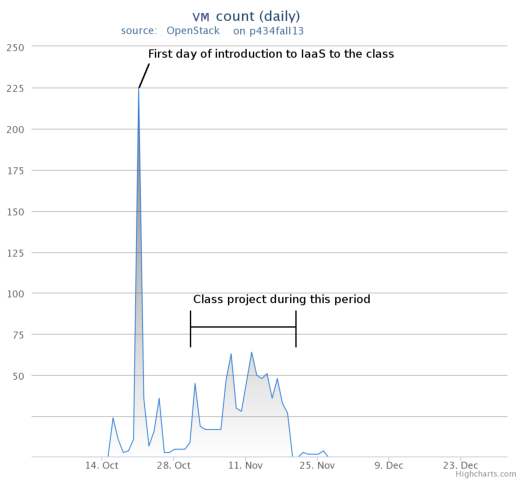
\includegraphics[width=1.0\columnwidth]{images/fig1.pdf} 
  \caption{The Architecture of the Framework}\label{F:fig1} 
\end{figure} 

\begin{figure}[htb] 
  \centering 
    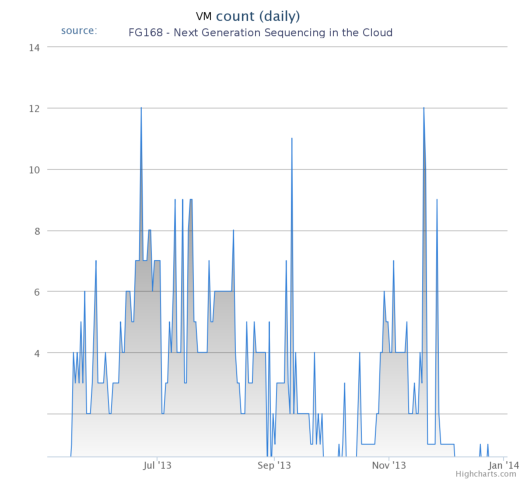
\includegraphics[width=1.0\columnwidth]{images/fig2.pdf} 
  \caption{The Architecture of the Framework}\label{F:fig2} 
\end{figure} 

\begin{figure}[htb] 
  \centering 
    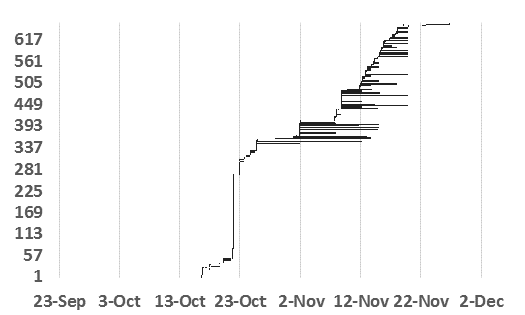
\includegraphics[width=1.0\columnwidth]{images/fig3.pdf} 
  \caption{The Architecture of the Framework}\label{F:fig3} 
\end{figure} 

\begin{figure}[htb] 
  \centering 
    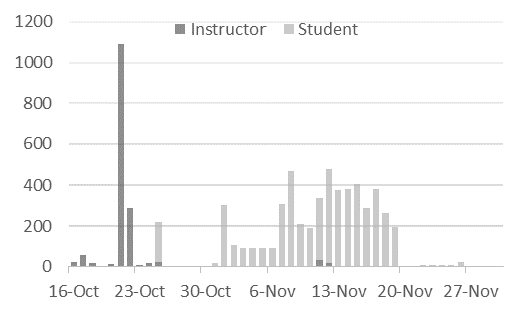
\includegraphics[width=1.0\columnwidth]{images/fig4.pdf} 
  \caption{The Architecture of the Framework}\label{F:fig4} 
\end{figure} 

\begin{figure}[htb] 
  \centering 
    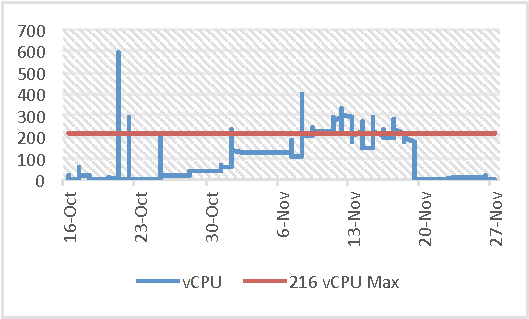
\includegraphics[width=1.0\columnwidth]{images/fig5.pdf} 
  \caption{The Architecture of the Framework}\label{F:fig5} 
\end{figure} 

\begin{figure}[htb] 
  \centering 
    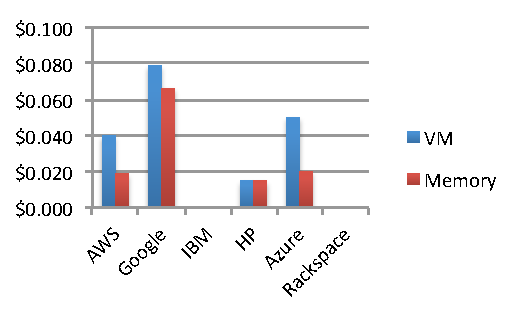
\includegraphics[width=1.0\columnwidth]{images/fig6.pdf} 
  \caption{The Architecture of the Framework}\label{F:fig6} 
\end{figure} 

\begin{figure}[htb] 
  \centering 
    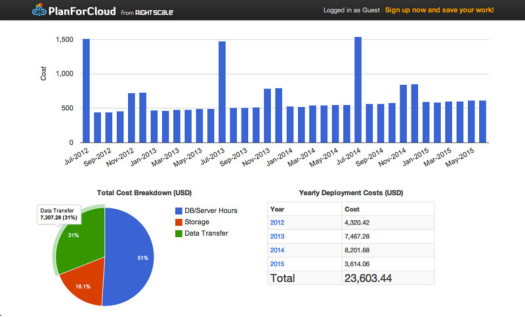
\includegraphics[width=1.0\columnwidth]{images/fig3b.pdf} 
  \caption{The Architecture of the Framework}\label{F:fig7} 
\end{figure} 

\begin{figure}[htb] 
  \centering 
    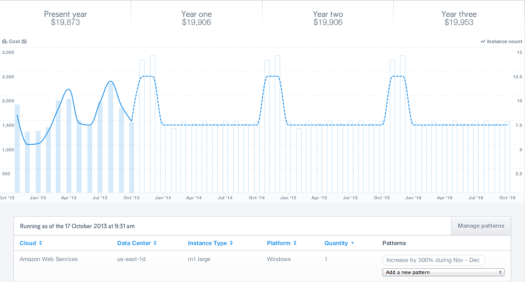
\includegraphics[width=1.0\columnwidth]{images/fig4b.pdf} 
  \caption{The Architecture of the Framework}\label{F:fig8} 
\end{figure} 


\section{BIG DATA}

With increasing the size of stored information in a rate of 23% per a year [20], the growth in the amount of educational and academic data means that data analysis, management and accessibility are going to be complicated to work with traditional data processing platforms and applications. Big Data is not only applied to the volume of data, but also applied to the length of the data life cycle [21] and variety, velocity, and veracity of the data [22]. In many areas such as meteorology, genomics, biological and environmental research [23, 24], researchers and educators need to process vast amounts of complex data instantly and accurately with analytical challenges. For example, Amazon Web Services and NASA work together to enable a large collection of NASA climate and Earth science satellite data to researchers and educators through Public Data Sets[?]. AWS Public Data Sets program is a centralized repository of large public data sets in an Elastic Block Storage or a Simple Storage Service (S3) format[?]. With the EBS snapshots, NASA NEX which is a large Earth science data sets can be easily attached to Amazon services i.e. Amazon Elastic Compute Cloud (Amazon EC2) for data analysis. 1000 human genomes to reveal DNA polymorphisms is also available through Amazon S3. The data sets have grown from small gigabytes to 200 terabytes.

\section{CAPABILITIES}

What is not met.

\section{USE CASE EXAMPLES}

\section{FutureGrid}

Based on the observation on FutureGrid, there is a different pattern between a research project and class work when they acquire cloud resources.  Resource allocation of academic coursework shows time dependent request patterns. It shows a surge when there is a class, a lab session, and a project. For example, the undergraduate course for Distributed Systems at Indiana University introduced IaaS in the class and used the IaaS platform for a class project. Figure 1 shows a spike in the class and variability until the project due. Research projects request VM instances in a bit more steady usage compared to the coursework. The Next Generation Sequencing (NGS) in the cloud project on FutureGrid shows relatively consistent resource allocation requested in Figure 2. With a certain period of time, vm instances of this project have been launched without unplanned spike requests. These examples show different patterns for requesting resources but both cases have a factor to predict loads. The class schedule and the monitoring and profiling data for applications can be used to measure the amount of resources and identify incoming requests. In paid cloud platforms such as AWS, GCE, and Azure, understanding these patterns for provisioning is important to bring cost effectiveness over on-demand allocation. For example, Amazon EC2 Reserved Instances and Azure pre-pay plans may help reduce usage costs for periodic and planned workloads. These service plans simply provide discounts with an upfront payment. As long as a class and a project go as planned, cost saving chances are increased. 

Figure 1. IaaS Usage data for the Distributed System class at Indiana University*

% * Based on the class schedule and metrics. Class schedule is here: http://salsahpc.indiana.edu/csci-p434-fall-2013/
% Metrics is here: http://129.79.49.94/accounting/reports/custom/p434fall13/FGResourceReport.pdf

 
Figure 2. VM count for Next Generation Sequencing (NGS) in the cloud project

With the Gantt chart in Figure 3, allocation activities are viewed for all virtual instances launched for the class. At the beginning of the class, the gaps between the start and completed dates of the vm instances are small but a large number of instances are initiated. Once the class is became operative,  running time for vm instances is getting longer and a smaller number of instances are requested compared to the beginning. This observation tells that academic projects require training sessions at the beginning of the project to get familiar with using infrastructure and to prepare environments by installing software and datasets.

 
Figure 3. Timeline for VM walltime

Other observation is that resource usage for administrative purposes. Figure 4 describes that instructors consumed a large number of vCPU cores before class starts and small tests just before class projects. It indicates that the preparation of courses require extensive load testing on cloud resources to estimate compute capacity needed for applications.

 
Figure 4. Usage between instructors and students for vCPU cores

During the semester, 25 hosts, 216 vCPUs and 600GB memories were reserved for the class since it required large virtual instances. In Figure 5 shows that the dedicated resources were being underutilized most time although the high volume requests had been made a few times including 273% overutilization on October 21th for testing and preparing.
 
Figure 5. vCPU Utilization (approximation per hour)

\section{OpenScience Grid}

\section{PlanetLab}

\section{COMPARISON}

QoS


% Overprovisioning
% Provider	Charging	Cost
% 1 vCPU /hour	Cost
% 1 GB
% /hour	OS	Max vCPU	Memory min - max	\# of instance types	Discount program	Free allowance
% Aws
% 	hourly	\$0.04
% 	$0.01927	Linux
% Windows +14-56% 
% Asia + 25%	32	615MB -
% 244GB	22	spot instance, 
% reserved instances	$100 for educator’s student
% Grant for researcher
% AWS educated grant program
% Google Compute Engine	10 minutes +
% every minute after that	$0.0788
% 	$0.006636
% 
% Europe + 4.5% - 27% 	Linux (Debian, CentOS)
% (RHEL, SUSE premium operating systems) ***	16	600MB -
% 104GB	15
% (4 high cpu + 4 high memory + 2 small + 5 standard)	n/a	Google app reward programs
% $1000 for educator
% $60,000 for research project
% IBM CloudLayer (by Softlayer)	monthly
% hourly	$0.5
% to
% $0.10	varies	Linux, 
% Windows + $0.05 to
%               $0.10 / hour	16	1GB 
% – 
% 64GB	Build your own cloud server offers customized options		one month trial for 1 vcpu + 1gb memory + 25 storage
% HP cloud	hourly	$0.015	$0.015	Linux, Windows, SUSE
% (windows: 10-200% extra charge,
% SUSE: 4% - 200% extra charge)	16	1GB 
% – 
% 120GB	11 (8 standard + 3 memory intensive)		$300 free trial for 90 days ($100 for each month)
% Microsoft Azure	Free first 5 minutes
% 	$ 0.05	$0.02 (approx.)
% Windows is expensive 30-50% more than linux	Linux, 
% Windows + 30-50% 	8	768MB – 
% 56GB	8 (A0-A7)	6-Month, 12-month pre-pay membership	$200 free trial of first month
% Rackspace	minute		varies	Linux, Windows
% (windows: 25% extra charge)	32	1GB – 
% 120GB	9	Volume discount (4% to 20% for spending over $5,000 - $ 10, 000 per month, 8% for $10,001 - 30,000, 12% for $30,001 - $50,000)
% Commitment discount (4% to 40%)
% Prepayment discount with commitment (7% to 55%)	$300 developer discount ($50 each for six months)
% Outage
% Expectations on quality

Comparison between iaas platforms?
Show changes from euca to openstack?

\section{FOR PAY ALLOCATIONS}

It has been made clear by the many cloud providers that the use of cloud data centers provides an economical advantage for the organization as the overall cost model that not only includes the 

\section{WHICH CLOUDS TO CONSIDER?}

\subsection{IaaS Cloud EC2 like services}
Charge. 
1.	find refernces and include here (properly, academic refernces, with pages to wher stuff is charged
2.	identify similarities and differences. For example google charges 15 min and after that every minute, AWS charges for an hour even if you just use a second
3.	

1)	AWS
*	http://aws.amazon.com/tco-calculator/
*	http://calculator.s3.amazonaws.com/calc5.html
*	http://aws.amazon.com/pricing/
*	spotpricing



\subsection{Pricing Comparison in IaaS}

Comparing pricing of the cloud is complicated and may lead to false analogy because each cloud provider offers various services with different performance. The pricing comparison, however, is important when people start to consider adopting cloud services among a lot of selections from different providers. In the comparison, important criteria are revealed through its pricing table. For example, there are a range of service offered, a size of available systems, costs, discounts and benefits such as technical support, and development tools. Amazon AWS, Windows Azure, Google Compute Engine, HP Cloud, IBM and Rackspace are compared.

 

 

 

\subsection{Example of pricing comparison}

We tried to apply each pricing model; Amazon AWS, Google Compute Engine, Microsoft Azure; to the usage data of class (P434 distributed systems at Indiana University), to compare cost estimate of cloud resource. Google Compute Engine is the least expensive and 16\% lower than Amazon AWS. It is mostly because of that Google has 10\% discount pricing chart compared to AWS. We observed that a minute basis charge is only 3.3\% less expensive for this class. Some restrictions and offers such as Google’s 10-minute minimum charge and Azure’s less 5-minute free of charge are relatively small amount of a discount or an extra charge. Google’s 10-minute minimum charge asks 0.18\% extra charge to the class, Azure provides 0.05\% discount through their less 5-minute free of charge. Amazon only has an hourly based pricing model, while Google Compute Engine and Windows Azure offer a minute basis charge for use of virtual machine instances. Three types of instances (small/medium/large) had been used for its coursework and projects and usage of virtual machine instances was only calculated without network and storage usage. Table 3, 4 shows pricing comparison to the class.

Table 3. Usage data of the class

Instance types	Instance count	Hour basis	Minute basis	With Google 10-minute minimum charge	with Azure 5-minute free
small	165	619 hrs (37,140 mins)	29,622 mins	29,875 mins	29,582 mins
medium	6	268 hrs (16,080 mins)	15,891 mins	15,891 mins	15,891 mins
large	490	10,831 hrs (649,860 mins)	629,969 mins	631,047 mins	629,667 mins
Total	661	11,718 hrs (703,080 mins)	675,482 mins	676,813 mins	675,140 mins
* Instance types are not same. Chosen by a similarity of vCPU and Memory
** Captured by January, 2014

Table 4. Pricing comparison to the class
Service	Cost Estimate	Pricing (Small/Medium/Large)	Restriction
AWS	$2,668.74	$0.06\$0.12\$0.24 per hour (US East Region, Linux)	Hour basis charge
GCE	$2,231.54	$0.054\$0.104\$0.207 per hour (US Region, Linux)	Minute basis charge with 10-minute minimum
Azure	$2,580.03	$0.06\$0.12\$0.24 per hour (Linux)	Minute basis charge with 5 less minute free

Charging model describe in text how they cjhharge and for what, e.g. what do they offer

1)	HP Cloud

2)	Google
3)	Rackspace
4)	IBM
5)	IBM

heruko vs amazon
% http://www.smashingboxes.com/heroku-vs-amazon-web-services/


Supported by libcloud
*	http://www.abiquo.com
*	http://brightbox.com
*	https://www.gandi.net/hosting/iaas/livemigration
*	http://www.vr.org
*	https://www.linode.com
*	https://www.bluebox.net
*	http://www.cloudsigma.com
*	https://www.digitalocean.com
*	dreamhost
*	http://www.elastichosts.com
*	gogid
*	gridspot
*	hostvirtual
*	ibm\_SCE
*	joynet
*	ktucloud
*	ninefold
*	opsource
*	rimuhosting
*	serverlove
*	skalicloud
*	slicehost
*	softlayer
*	voxel
*	vpsnet
*	bitnami?
*	
\subsection{Comparison}

Table 1. Pricing chart for instances from AWS, GCE, and Azure
	Billing granularity	Price	Variation for Price
AWS	By hour	\$0.02 (smallest)*	10 regions**, 6 platforms
GCE	By minute, with a minimum of 10 minutes	\$0.019 (smallest)*	2 regions (Us, Europe)
Azure	By minute, No minimum, No billing for less than 5 minutes	\$0.02 (smallest)*	6 regions, 5 platforms
* Smallest VM instance: 1 virtual core, 600~768MB memory, no storage
** China (Beijing) region will be available in early 2014, and GovCloud region is also included.

Pricing is scenario based. It can’t be simply compared with numbers. GCE looks cheaper than other competitors, but others have more options to save a cost. For example, a pay-ahead model provides a discount for same instances, and a spot instance also provides a way of saving entire cost for task intensive workloads in a small amount of time.


\subsection{Tools for Cloud Pricing}

To help understand costs of cloud computing, several tools offer various functions to calculate estimate and analyze cloud spending and usage data. With these tools, researchers and educators can make a plan for cloud deployments and prepare spending across several cloud providers. Each cloud service consists of complicated architectures and different performance levels and so users need to understand that these tools for cloud pricing are designed to minimize costs and provide guidelines in terms of finding the most effective cloud services.

1. PlanForCloud Calculator
PlanForCloud Calculator is a free cloud cost forecasting website that
helps evaluate costs for a project or an operation from a variety of
cloud providers. With PlanForCloud, Amazon Web services (AWS), Google
Compute Engine (GCE), Microsoft Windows Azure, Rackspace, IBM
Softlayer, and HP Cloud are compared for servers, storage, databases,
data transfer, and other services to estimate resource usage in the
future. This calculator also provides a simulation on planned
deployments and 3-year cost reports. Estimated expenditures can be
illustrated to reduce uncertainty for the future consumption of cloud
resources. 

% [http://www.rightscale.com/news_events/press_releases/2012/rightscale-introduces-cloud-cost-forecasting-with-launch-of-planforcloud.php]

[Helen Heinrich (2013) Tech Servises on the Web: The PlanforCloud
Calculator http://www.planforcloud.com/ , Technical Services Quarterly, 30:1, 120-121, DOI:
10.1080/07317131.2013.735980]

 
Figure 3. Example of a cloud usage report by PlanForCloud from RightCcale **

** screenshot from http://www.rightscale.com/images/pfc-report-page.jpg


 
Figure 4. Example of Cloud Analytics from Rightscale***

***screenshot from http://www.rightscale.com/images/screenshots/cloud-cost-forecasting.png

We can not compare all the things, so we need to identify a subset for comparision, what should we compare

Tiny, small, medium, lareg mage of comparable size

Create graph with entry for each type with y axis on some metric we can compare this will create a “band” on y but have a single entry for each IaaS. 

goalsCan accost model be derived for each cloud given some parameters



*	http://www.profitbricks.com/compare-cloud-pricing/
%*	https://cloudvertical.com/cloud-costs#cloud_costs/index
*	http://mikekhristo.com/ec2-ondemand-vs-reserved-instance-savings-calculator/
*	http://blog.cloudphysics.com/blog/2013/11/18/do-hybrid-clouds-make-cents-free-cost-calculator-for-aws
*	http://geekswithblogs.net/hroggero/archive/2013/02/18/sample-pricing-comparison-amazon-aws-and-windows-azure.aspx
*	http://www.stratalux.com/2013/05/08/strataluxs-aws-pricing-tool/
*	http://www.webrmedia.com/blog/apps/calculate-your-amazon-aws-hosting-costs-using-excel

D.	PaaS
1)	AWS service xyz
2)	???




\section{Tools}

1)	Management Tools
Rightscale
2)	Metric systems
Rightscale, 
….pulbic clouds that monitor your AWS or other cloud


\section{Citations}

just to show whats in cyberaide-metrics.bib

\cite{www-c,www-b,www-a,www-abc,www-salsa-class,www-amzon-calculator2,www-o,www-n,www-m,www-l,www-k,www-j,www-i,www-h,www-g,www-f,www-w,www-v,www-u,www-t,www-s,www-r,www-q,www-p,www-e,www-d,www-amzon-calculator-1,www-amzon-calculator-2}
 

 
%%%%%%%%%%%%%%%%%%%%%%%%%%%%%%%%%%%%%%%%%%%%%%%%%%%%%%%%%%%%%%%%%%%%%% 
% Acknowledgment 
%%%%%%%%%%%%%%%%%%%%%%%%%%%%%%%%%%%%%%%%%%%%%%%%%%%%%%%%%%%%%%%%%%%%%% 
  
\section*{Acknowledgement} 
 
This material is based upon work supported in part by the National Science Foundation under Grant No. 0910812.

 
%\clearpage 
 
\bibliographystyle{IEEEtranS} 
%\bibliographystyle{abbrv} 
\bibliography{% 
bib/vonLaszewski-jabref,% 
bib/cyberaide-metric,%
bib/cyberaide-cloud}
%bib/image-refs,% 

%bib/python,% 
%tas.bib%
 
\end{document} 
 
 
